%% Copyright 2015 M. Harland
  %
  % This work may be distributed and/or modified under the
  % conditions of the LaTeX Project Public License, either version 1.3
  % of this license or (at your option) any later version.
  % The latest version of this license is in
  %   http://www.latex-project.org/lppl.txt
  % and version 1.3 or later is part of all distributions of LaTeX
  % version 2005/12/01 or later.

%%%%%%%%%%
\documentclass[12pt,a4paper]{article}

\usepackage[left=2.5cm,right=2.5cm,top=1.0cm,bottom=2cm]{geometry}
\usepackage{placeins}

%\usepackage{graphicx}
%\usepackage{subcaption}
%\usepackage{amsmath}
%\parindent=1cm
%%%%%%%%%



%\marginparwidth = 0pt
%\hoffset = 0pt
%\oddsidemargin = 0pt
%\marginparsep = 0pt
%\voffset = 0pt

%\documentclass{amsproc}
%\documentclass[11pt,
%paper=a4,
%bibtotocnumbered,	  % Literaturverzeichnis ins Inhaltsverzeichnis
%liststotocnumbered,  % Alle Listen ins Inhaltsverzeichnis							
%DIV=calc,		  % führt die Satzspiegelberechnung neu aus
%oneside,		  % einseitiger Druck
%tablecaptionabove,	  % Tabellenüberschriften aktivieren
%BCOR=16mm,	  % Bindekorrektur
%headinclude,
%footinclude
%]{article}


%%%%
%\usepackage{fancyhdr}
%\usepackage{lipsum} % only for showing some sample text
%\fancyhf{} % clear all header and footers
%\renewcommand{\headrulewidth}{0pt} % remove the header rule
%\rfoot{\thepage}
%\pagestyle{fancy}
%\usepackage{indentfirst} % Красная строка
%%%%




\usepackage{amssymb}
\usepackage{amsmath}
\usepackage{graphicx}
\usepackage{color}
\def\x{{\bf x}}
\def\y{{\bf y}}
\newcommand{\XY}[1]{\textcolor{magenta}{X$\rightarrow$ Y: #1}}

\usepackage{mathrsfs,bbm}
\usepackage{comment}
\newcommand{\bm}[1]{\boldsymbol #1}
\newcommand{\lh}{\mbox{$\neg$}}
\newcommand{\rh}{\reflectbox{$\neg$}}
\usepackage{txfonts}
\DeclareSymbolFont{symbols}{OMS}{cmsy}{m}{n}
\DeclareSymbolFont{largesymbols}{OMX}{cmex}{m}{n}

%%%%%%%%%%%%%%%%%%%%%%%%%%%%%%%%%%%%%%%%%%%%%%%%
%Genaral math symbols
\newcommand{\TR}{\text{Tr}}
\newcommand{\BK}{{\bm k}}
\newcommand{\Vk}{{\bm k}}
\newcommand{\Ks}{{{\bm k}\sigma}}
\newcommand{\tb}{{\bar t}}
\newcommand{\myast}{{{}\hspace*{-0.1em}\ast\hspace*{-0.1em}{}}}
\newcommand{\mydagger}{{\dagger}}
\newcommand{\phdagger}{{\phantom{\dagger}\!}}
\newcommand{\bra}[1]{\langle{#1}|}
\newcommand{\ket}[1]{|{#1}\rangle}
\newcommand{\braket}[2]{\langle{#1}|{#2}\rangle}
\newcommand{\expval}[1]{\langle{#1}\rangle}
%%%%%%%%%%%%%%%%%%%%%%%%%%%%%%%%%%%%%%%%%%%%%%%%
%Contour calculus notation
\newcommand{\CS}{\mathcal{S}}
\newcommand{\ii}{^j}
\newcommand{\delC}{\delta_\CC}
\newcommand{\intC}{\int_\CC}
\newcommand{\tmin}{t_{\text{min}}}
\newcommand{\tmax}{t_{\text{max}}}
\newcommand{\CC}{\mathcal{C}}
\newcommand{\TC}{\mathcal{T}_{\CC}}
\newcommand{\gtrc}{\succ}
\newcommand{\lesc}{\prec}
%%%%%%%%%%%%%%%%%%%%%%%%%%%%%%%%%%%%%%%%%%%%%%%%
%Keldysh Green functions
\newcommand{\convz}{\ast}
\newcommand{\convi}{\bullet}
\newcommand{\convr}{\circ}
\newcommand{\ret}{{\text{R}}}
\newcommand{\adv}{{\text{A}}}
\newcommand{\mat}{{\text{\tiny M}}}
\newcommand{\tv}{{\makebox{$\neg$}}}
\newcommand{\vt}{{\reflectbox{$\neg$}}}
\newcommand{\les}{<}
\newcommand{\lar}{>}
%%%%%%%%%%%%%%%%%%%%%%%%%%%%%%%%%%%%%%%%%%%%%%%%
%misc
\newcommand{\ETAL}{{\em et al.}}
\newcommand{\Ucdyn}{{U_{\text{dyn}}}}
\newcommand{\sss}{_{\alpha\alpha'}}
\newcommand{\YY}{Y}
\newcommand{\KK}{K}
\newcommand{\pseudo}{\widetilde}
\newcommand{\cyles}{\prec}
\newcommand{\scell}{\text{scel}}
\newcommand{\pG}{\mathcal{G}}
%%%%%%%%%%%%%%%%%%%%%%%%%%%%%%%%%%%%%
%FK
\newcommand{\Gwnull}{Q}\newcommand{\Gweins}{R}
\newcommand{\gwnull}{q}\newcommand{\gweins}{r}
%%%%%%%%%%%%%%%%%%%%%%%%%%%%%%%%%%%%%
% for Mott Breakdown
\renewcommand{\dh}{dh}
\newcommand{\jd}{\Gamma_\text{\dh}}
\newcommand{\fth}{F_\text{th}}
\newcommand{\hopp}{{t^*}}
\renewcommand{\bar}{\overline}

%\input{defs}
\newcommand{\cis}{c_{i\sigma}}
\newcommand{\cisd}{c_{i\sigma}^\dagger}
\newcommand{\cs}{c_{\sigma}}
\newcommand{\csd}{c_{\sigma}^\dagger}
\newcommand{\cst}{c_{\sigma}(\tau)}
\newcommand{\csdtp}{c_{\sigma}^\dagger(\tau')}
\newcommand{\nup}{n_{\uparrow}}
\newcommand{\ndown}{n_{\downarrow}}
\newcommand{\nupt}{\nup(\tau)}
\newcommand{\ndownt}{\ndown(\tau)}
\newcommand{\nuptp}{\nup(\tau')}
\newcommand{\ndowntp}{\ndown(\tau')}
\newcommand{\nuptpp}{\nup(\tau'')}
\newcommand{\ndowntpp}{\ndown(\tau'')}
\newcommand{\nupti}{\nup(\tau_i)}
\newcommand{\nupta}{\nup(\tau_1)}
\newcommand{\ndownti}{\ndown(\tau_i)}
\newcommand{\ndownta}{\ndown(\tau_1)}
\newcommand{\nuptj}{\nup(\tau_j)}
\newcommand{\nuptb}{\nup(\tau_2)}
\newcommand{\ndowntj}{\ndown(\tau_j)}
\newcommand{\ndowntb}{\ndown(\tau_2)}
\newcommand{\nuptk}{\nup(\tau_k)}
\newcommand{\ndowntk}{\ndown(\tau_k)}
\newcommand{\Tr}{\text{Tr}}
\newcommand{\Hloc}{H_\text{loc}}
\newcommand{\Hhyb}{H_\text{hyb}}
\newcommand{\Hhybtwid}{\tilde{H}_\text{hyb}}
\newcommand{\fatx}{\mathbf{x}}
\newcommand{\fatX}{\mathbf{X}}
\newcommand{\fatk}{\mathbf{k}}
\newcommand{\fatK}{\mathbf{K}}
\newcommand{\fattildek}{\mathbf{\tilde{k}}}
\newcommand{\fattildex}{\mathbf{\tilde{x}}}
\newcommand{\fatt}{\mathbf{t}}
\newcommand{\fatg}{\mathbf{g}}
\newcommand{\fatG}{\mathbf{G}}
\newcommand{\fatbarG}{\mathbf{\overline{G}}}
\newcommand{\fatmathcalG}{\mathbf{\mathcal{G}}}
\newcommand{\fatSigma}{\mathbf{\Sigma}}
\newcommand{\vk}{{\mathbf{k}}}
\newcommand{\N}{{\mathbf{N}}}
\newcommand{\G}{{\mathbf{G}}}
\newcommand{\D}{{\mathbf{D}}}
\newcommand{\M}{{\mathbf{M}}}
\newcommand{\fatP}{{\mathbf{P}}}

\def\stau{\{ s_{i},\tau_{i}, x_i\}}
\def\staup{\{ s_{i}',\tau_{i}', x_i'\}}
\newcommand{\hyb}[2]{\Delta(\tau_{#1}^e-\tau_{#2}^s)}


\newcommand{\pa}{\partial}
\newcommand{\vphi}{\varphi}
\newcommand{\ve}{\varepsilon}
\newcommand{\up}{\uparrow}
\newcommand{\dw}{\downarrow}
\newcommand{\Vect}[1]{\mbox{\boldmath$#1$}}


% for introduction
\newcommand{\mb}[1]{\mathbf{#1}}
\newcommand{\mcl}[1]{\mathcal{#1}}
\newcommand{\al}{\alpha}
\newcommand{\be}{\beta}
\newcommand{\bz}{\bar{z}}
\newcommand{\e}{\epsilon}
\newcommand{\s}{\sigma}
\newcommand{\om}{\omega}
\newcommand{\la}{\lambda}
\newcommand{\bJ}{\bar{J}}
\newcommand{\brz}{\bar{z}}
\newcommand{\brq}{\bar{q}}
\newcommand{\vp}{\varphi}
\newcommand{\bvp}{\bar{\varphi}}
\newcommand{\tvp}{\tilde{\varphi}}
\newcommand{\hil}{\mcl{H}}
\newcommand{\vir}{\mathfrak{Vir}}
\newcommand{\no}{\nonumber}
\newcommand{\tr}{\mbox{Tr}}
\newcommand{\itl}{{\it l}}
\newcommand{\mbx}{\mathbf{x}}
\newcommand{\ihbar}{\frac{i}{\hbar}}



















%%%%
%\usepackage[utf8]{inputenc}
%\usepackage{graphicx} %includegraphics
%\usepackage{braket} %Bra and Ket
%\usepackage{amsmath} %mathcal etc
%\usepackage{natbib} %citep, citet, bib-style
%\usepackage[colorlinks]{hyperref}
%\newcommand{\mysubtitle}[1]{\section{#1}}
%\usepackage[usenames,dvipsnames]{xcolor}
%%%%
%\definecolor{persianplum}{rgb}{0.44, 0.11, 0.11}
%\definecolor{mulberry}{rgb}{0.77, 0.29, 0.55}
%\definecolor{maroon(html/css)}{rgb}{0.5, 0.0, 0.0}
%\definecolor{indigo(dye)}{rgb}{0.0, 0.25, 0.42}
\begin{document}
\title{Theory}
%\author{V.N. Valmispild}
\date{\today}
\maketitle
%\tableofcontents

\chapter{Nonequilibrium many-body theory}
\label{chap:Non_mb_th}

\section{Nonequilibrum Green's function approach}

There are different approaches to account for time dependencies in a quantum mechanical system with its advantages and disadvantages. One of the most popular is a Keldysh formalism for nonequilibrium Green's functions. Kadanoff and Baym \citep{bookKadanoff_and_Baym} introduced the concept of two real-time Green functions, thus developing the standard equilibrium (imaginary-time) formalism \citep{Abrikosov:107441} to nonequilibrium \citep{10.1063/1.1703727}. In this work, we use L-shaped Green contour functions, which were introduced by Keldysh \citep{Keldysh:1964ud} and Danilevich \citep{DANIELEWICZ1984239}. Many theoretical approaches that have been developed for the study of strongly correlated systems can be adapted for nonequilibrium systems using the Keldysh formalism.

\FloatBarrier

\subsection{Contour idea}
	
Time-dependent experimental measurements can be related with expectation values of observables $\langle{O(t)}\rangle$. An expectation value of a quantum mechanical operator $O$ at time $t$ given by 
\begin{align}
\langle O(t)\rangle
 &=
  Tr[\rho(t)O].
\label{expectation value}
\end{align}
where $\rho(t)$ is a time-dependent density matrix. 

Initial (at $t=0$) system is in a mixed state represented by a density operator
\begin{align}
\rho(0)
&=
  \frac{1}{Z}e^{-\beta H(0)},
\label{rho0}
\end{align}
where $H(t)$ - time-dependent Hamiltonian, $\beta=1/T$ is the inverse temperature, $Z={\rm Tr}\, e^{-\beta H(0)}$ is the thermal equilibrium partition function.
At $t=0$ we switch on a driving field, and the system starts to evolve from its initial state. 
A Neumann equation describes how the density operator evolves in time and has the following expression
\begin{align}
i\frac{d}{dt}\rho(t)
 &=
  [H(t),\rho(t)],
\label{von Neumann}
\end{align}
where the brackets denote a commutator. The solution for the equation can be written as 
\begin{align}
\rho(t)
&= U(t,0)\, \rho(0) \, U(0,t),
\label{formal rho}
\end{align}

where the interaction time evolution operator defined as
\begin{align}
U(t,t')
 &=
  \begin{cases}
   \vspace{.2cm}
   \displaystyle
   T \exp\left(-i\int_{t'}^t d\bar{t}\, H(\bar{t})\right) 
   & t>t'
   \\
   \displaystyle
   \bar{T} \exp\left(-i\int_{t'}^t d\bar{t}\, H(\bar{t})\right)
   & t<t'
  \end{cases}.
\label{U def}
\end{align}
Here $T$ denotes time-ordering and $\bar{T}$ anti-time-ordering operators. Operator $H(t)$ odered by operator $T$ such that the time
arguments $\bar{t}$ increase from right to left and vice versa for $\bar{T}$. The density matrix involves one exponent with a forward integration along the time axis due to $U(t,t')$, one with a backwards integration due to $U(t',t)$, and in initial state with $exp(- \beta H(0))$.
\begin{figure}[h!]
\center{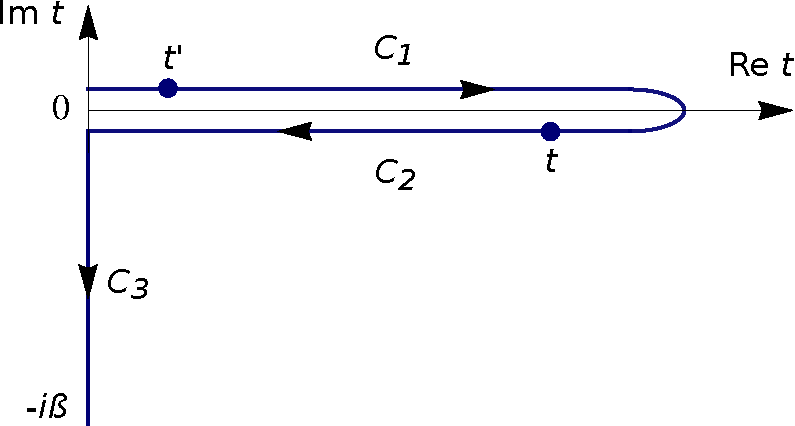
\includegraphics[width=0.5\linewidth]{Chapters/Theory_Kelgysh/figure/kadanoff-baym_contour.pdf}} 
\caption{L-shaped contour}
\label{L-shaped contour}
\end{figure}

	
Finally, the time-dependent expectation value with respect of initial equilibrium and the time-dependent density matrix can be expressed as
\begin{align}
\left\langle O(t) \right\rangle =\dfrac{1}{Z}
Tr\left[ U(-i \beta,0) U(0,t) O U(t,0) \right] =
\dfrac{Tr\left[ T_C e^{-i \int_C d \hat{t} H(\hat{t}) O(t) } \right] }{Tr\left[ T_C e^{-i \int_C d \hat{t} H(\hat{t})} \right] }
\label{expectation value2}
\end{align}
where $T_{C}$ is a contour-ordering operator that organize operators on the contour $C$ in the order 
 $0 \rightarrow t_{max} \rightarrow 0 \rightarrow -i \beta$ (Fig.~\ref{L-shaped contour}), $O(t)$ indicates that the operator $O$ is inserted at time $t$ on the contour $C$ \citep{bookKadanoff_and_Baym}.
 
Such time parametrization along the contour allows us to derive many techniques from equilibrium many-body theory to nonequilibrium. 
It should be noted that other time contours can also be used depending on the physical situation.


	
\FloatBarrier
\subsection{Contur-ordered Green's functions and self-energy}
	
One particle contour-ordering Green's functions is defined according to
\begin{align}
G(t,t')
&\equiv
-i\langle T_{C}\, c(t)\, c^\dagger(t')\rangle,
\label{green def}
\end{align}

where $c^{\dagger}$($c$) is a creation (annihilation) operator of particles, and $t,t' \in C$. Spin and orbital indices are not shown to simplify writing equations.

The contour $C$ is divided into three branches $C_1$, $C_2$ and $C_3$ as in Fig.~\ref{L-shaped contour}. there are nine possibilities to distribute the arguments along the contour, which can be grouped in a $(3 \times 3)$ matrix \citep{PhysRevB.44.6104}. 

Each component of the Green's functions satisfies
\begin{subequations}
\begin{align}
 \label{redundancy-1}
 G^{11}(t,t')
  &=
   G^{12}(t,t') \quad ({\rm for}\; t\le t'),
 \\
 G^{11}(t,t')
  &=
   G^{21}(t,t') \quad ({\rm for}\; t>t'),
 \\
 G^{22}(t,t')
  &=
   G^{21}(t,t') \quad ({\rm for}\; t<t'),
 \\
 \label{redundancy-4}
 G^{22}(t,t')
  &=
   G^{12}(t,t') \quad ({\rm for}\; t\ge t'),
 \\
 G^{13}(t,\tau ')
  &=
   G^{23}(t,\tau '),
 \\
 G^{31}(\tau,t')
  &=
   G^{32}(\tau,t').
\end{align}
\label{redundancy}
\end{subequations}


Some components can be summarized as
\begin{align}
G^{11}(t,t')+G^{22}(t,t')
 &=
  G^{12}(t,t')+G^{21}(t,t'). 
\label{linear dependence1}
\end{align}

But such matrix representation is overcomplete because not all components are independent. One can reduce $(3 \times 3)$ matrix using linear transformation (Keldysh rotation),
\begin{align}
 \hat{G}
  &=
   \begin{pmatrix}
    G^{R} & G^{K} & \sqrt{2} G^{\lh} \\
    0 & G^{A} & 0 \\
    0 & \sqrt{2} G^{\rh} & G^{M}
   \end{pmatrix}
   =L\tau_3
   \begin{pmatrix}
    G^{11}(t,t') & G^{12}(t,t') & G^{13}(t,\tau ') \\
    G^{21}(t,t') & G^{22}(t,t') & G^{23}(t,\tau ') \\
    G^{31}(\tau,t') & G^{32}(\tau,t') & G^{33}(\tau,\tau')
   \end{pmatrix}L^{\dagger}.
 \label{G_3x3}
\end{align}
where rotating $L$ and Pauli $\tau_3$ matrices,
\begin{align}
 L
  &=\frac{1}{\sqrt{2}}
   \begin{pmatrix}
    1 & -1 & 0 \\
    1 & 1 & 0 \\
    0 & 0 & \sqrt{2}
   \end{pmatrix}
    , \: \: \: \: \tau_3=
   \begin{pmatrix}
    1 & 0 & 0 \\
    0 & -1 & 0 \\
    0 & 0 & 1
   \end{pmatrix}.
 \label{rotating_pauli}
\end{align}

Thus, only six linearly independent Greens functions remain. They are called as retarded ($G^R$), advanced ($G^A$), Keldysh ($G^K$), left-mixing ($G^{\lh}$), right-mixing ($G^{\rh}$), and Matsubara Green's function ($G^M$). They can be parameterized as follows
\begin{subequations}
\label{physical green def}
\begin{align}
G^R(t,t')
 &=
   \tfrac12(G^{11}(t,t')-G^{12}(t,t')+G^{21}(t,t')-G^{22}(t,t'))
\nonumber
\\
 &=
  -i\theta(t-t') \langle [c(t),c^\dagger(t')]_\mp \rangle,
\\
G^A(t,t')
 &=
   \tfrac12(G^{11}(t,t')+G^{12}(t,t')-G^{21}(t,t')-G^{22}(t,t'))
\nonumber
\\
 &=
  i\theta(t'-t) \langle [c(t),c^\dagger(t')]_\mp \rangle,
\label{advanced green def}
\\
G^K(t,t')
 &=
   \tfrac12(G^{11}(t,t')+G^{12}(t,t')+G^{21}(t,t')+G^{22}(t,t'))
\nonumber
\\
 &=
  -i \langle [c(t),c^\dagger(t')]_\pm \rangle,
\label{keldysh green function}
\\
G^{\lh}(t,\tau ')
 &=
   \tfrac12(G^{13}(t,\tau ')+G^{23}(t,\tau '))
 =
   \mp i \langle c^\dagger(\tau ') c(t) \rangle,
\\
G^{\rh}(\tau, t')
 &=
   \tfrac12(G^{31}(\tau,t')+G^{32}(\tau,t'))
 =
   -i\langle c(\tau) c^\dagger(t') \rangle,
\\ \:
\:G^M(\tau,\tau ')
 &=
   -iG^{33}(\tau,\tau')
 =
   -\langle \mathcal{T}_\tau\, c(\tau) c^\dagger(\tau ') \rangle.  
\end{align}
\end{subequations}

Correlation functions $G^{>}$ and $G^{<}$ which correspond propagation of a "particle" and a "hole":
\begin{align}
\label{gles def}
 G^<(t,t')
  &=
   G^{12}(t,t')
  =
   \mp i \langle c^\dagger(t') c(t) \rangle
  = \tfrac12
   (G^K(t,t')-G^R(t,t')+G^A(t,t')),  
 \\
\label{ggtr def}
 G^>(t,t')
  &=
   G^{21}(t,t')
  =
   -i \langle c(t) c^\dagger(t') \rangle
  = \tfrac12
   (G^K(t,t')+G^R(t,t')-G^A(t,t')).
\end{align}

Using the above contur-ordered Green's function one can rewrite as inverse adopting for noninteracting tight-binding Hamiltonian $H_0(t)=\sum_k[\epsilon_k(t)-\mu]c_k^\dagger c_k$:
\begin{align}
\label{G0inv_k}
G^{-1}_{0,k}(t,t')=[i\partial_t+\mu -\varepsilon_k(t)]\delta_C(t,t')
\end{align}
where $\delta_C(t,t')=\partial_t \theta_C(t,t')$.

It is possible to describe the many-body interactions of a single particle by introducing an energy dependent effective potential called self-energy ($\Sigma$). Similar to the Green's functions the self-energy is defined on the L-shaped contour and has a $(3 \times 3)$ matrix structure which can be reduced using the Keldysh rotation \citep{PhysRevB.44.6104}:
\begin{align}
 \hat{\Sigma}
  &=
   \begin{pmatrix}
    \Sigma^{R} & \Sigma^{K} & \sqrt{2} \Sigma^{\lh} \\
    0 & \Sigma^{A} & 0 \\
    0 & \sqrt{2} \Sigma^{\rh} & \Sigma^{M}
   \end{pmatrix}
   =L\tau_3
   \begin{pmatrix}
    \Sigma^{11}(t,t') & \Sigma^{12}(t,t') & \Sigma^{13}(t,\tau ') \\
    \Sigma^{21}(t,t') & \Sigma^{22}(t,t') & \Sigma^{23}(t,\tau ') \\
    \Sigma^{31}(\tau,t') & \Sigma^{32}(\tau,t') & \Sigma^{33}(\tau,\tau')
   \end{pmatrix}L^{\dagger}.
 \label{S 3x3}
\end{align}
These components are called as retarded ($\Sigma^R$), advanced ($\Sigma^A$), Keldysh ($\Sigma^K$), left-mixing ($\Sigma^{\lh}$), right-mixing ($\Sigma^{\rh}$), and Matsubara ($\Sigma^M$).

The self-energy operator is related to the bare $G_0$ and dressed $G$ propagators and via the Dyson equation: 
\begin{align}
\label{dyson1}
\hat{G} = \hat{G_0} + \hat{G_0} \convz \hat{\Sigma} \convz \hat{G}.
\end{align}
where $*$ denotes convolution. Using a differential form for $G_0^{-1}$ this expression can be rewritten for various components as
\begin{align}
\label{dyson2}
&[i\partial_t - \mu +\varepsilon_k(t) ] G(t,t') - \int_\CC \!d\bar t\, \Sigma(t,\bar t) G(\bar t,t') 
= \delta_\CC(t,t')
\end{align}
From the physical point of view, the solutions of this equation describe the time-dependent single-particle spectrum $(G^R)$ and particle distribution $(G^<)$.


\FloatBarrier

\section{Hubbard model}
\label{section:Hubbard_model}
In 1960s the Hubbard model was proposed by Hubbard \citep{doi:10.1098/rspa.1963.0204}, Gutzwiller \citep{PhysRevLett.10.159} and Kanamori \citep{1963PThPh..30..275K} to describe electrons in $3d$ transition metal monoxides (FeO, NiO, CoO). 

The Hubbard model is one of the most important models in theoretical physics due to its simplicity and the number of physical phenomena that it can describe. These phenomena include metal-insulator transition, antiferromagnetism, ferrimagnetism, ferromagnetism, and superconductivity. 
Hamiltonian for single-band Hubbard model with time-dependent hopping amplitudes and local Coulomb repulsion,
\begin{subequations}
\begin{align}
\label{Habbard_Hamiltonian}
&
H(t)=H_{kin}(t)+H_{pot}(t)
\\
\label{Habbard_Hamiltonian_kin}
&
H_{kin}(t)=\sum_{ij\sigma} {t_{ij}(t)c^{\dagger}_{i \sigma} c_{j \sigma}}
\\
\label{Habbard_Hamiltonian_pot}
&
H_{pot}(t)=U(t) \sum_i{(n_{i\uparrow}-\frac{1}{2})(n_{i\downarrow}-\frac{1}{2})}
\end{align}
\end{subequations}
where $c^{\dagger}_{i \sigma}(c_{j \sigma})$ are creation (annihilation) operators for an electron with the spin $\sigma$ in the orbital at the lattice site $i$, $n_{i\sigma}=c^{\dagger}_{i \sigma} c_{j \sigma}$ counts the number of electrons with the spin $\sigma$ in the orbital at site $i$. The kinetic energy $H_{kin}(t)$ allows for tunneling of particles between sites of the lattice with amplitudes $t_{ij}(t)$. Potential term of the Hamiltonian $H_{pot}(t)$ corresponds of an on-site Coulomb interaction.

Due to recent growth of experimental interest in the systems driven out of equilibrium, such as the ultrafast pump-probe spectroscopies, theoretical methods to study such correlated systems are necessary. Thus, in later chapters, we will investigate the behavior of the Hubbard model out of equilibrium under the action of an external electromagnetic field. To do this, we describe the external spatially uniform electric field via the vector potential ${\bf A}(t)$
\begin{align}
\label{Vector_potential}
{\bf E(t)} = -\partial{\bf A}(t)/\partial t
\end{align}

The Peierls substitution \citep{Peierls1933} is used to account for the electric field in the Hamiltonian, so the hopping matrix in the general case elements satisfy
\begin{align}
\label{hoppings_1}
t_{ij}(t)=t_{ij}exp \left(-\int_{{\bf R}_i}^{{\bf R}_j} d{\bf r} {\bf A}({\bf{r}},t)\right)  
\end{align}

For the tight-binding parametrization of the electronic structure of the $CuO$ plane, which is a common feature of high-$T_c$ superconducting materials, we use the following dispersion law for a square lattice in the $k$-space:
\begin{subequations}
\begin{align}
\label{dispersion_1}
\varepsilon_1(k,t)
&=
{2t_1(cos(k_x+ A_x(t))+cos(k_y+A_y(t)))},
\\
\label{dispersion_2}
\varepsilon_2(k,t)
&=
	2t_1(cos(k_x+A_x(t))+cos(k_y+A_y(t)))
		\nonumber
		\\
 &+
4t_2(cos(k_x+A_x(t))\cdot cos(k_y+A_y(t))).
\end{align}
\end{subequations}
where $\varepsilon_1(k,t)$ corresponds to nearest neighbor (NN) approximation and $\varepsilon_2(k,t)$ next nearest neighbor (NNN).

Due to the fact that DMFT becomes exact in the limit of lattices with an infinite coordination we use for benchmarks the Bethe lattice with semielliptic density of states:
\begin{align}
\label{Bethe_lattice}
\rho(\varepsilon)=\dfrac{2\sqrt{1-(\varepsilon/D)^2}}{\pi D}
\end{align}
where $D$ is half-bandwidth.

The model has two extreme cases: 1) Limit with $U\rightarrow 0$ is a tight-binding model which entirely analogous for the investigation of spinless free fermions; 2) Limit with $t\rightarrow 0$ is called atomic limit where the electrons can not move, such case represent the Mott insulator.

\FloatBarrier

\section{ Nonequilibrium dynamical mean-field theory}
\label{section:NE_DMFT}
In equilibrium, the DMFT \citep{RevModPhys.68.13} plays a large role in understanding systems with strong electron correlations. An example of such DMFT success is explanation transition between a metal and the Mott insulator, and in combination with other theories for realistic simulation of many correlated materials. 

This chapter presents the nonequilibrium dynamical mean-field theory (NE-DMFT) \citep{RevModPhys.86.779} which allows studying the strongly correlated many-body systems out of equilibrium. 


\FloatBarrier
\subsection{Self-consistency loop}
An approximation of equilibrium and out of equilibrium DMFT is the local nature of the self-energy. This means that self-energy is momentum-independent.
\begin{equation}
\Sigma_{ij}^\text{lat}(t,t')\approx \delta_{ij}\Sigma^\text{imp}(t,t').
\end{equation}
This fact allows mapping of a lattice problem to a self-consistent solution of a quantum impurity model, which is exact in the limit of infinite dimensions. 
We can write nonequilibrium single-site action as
\begin{align}
\label{Action}
S_{imp}=-i\int_C dt H_{pot}(t)-i\sum_{\sigma}{\int_C dt dt' c^{\dagger}_{\sigma}(t) \Delta_i (t,t') c_{\sigma}(t')}
\end{align}
where $\Delta_i (t,t')$ is time-dependent hybridization function wich represents the hopping amplitude from the impurity into the bath \citep{PhysRevB.45.6479}.

After that we can define the contour-ordered impurity Green’s function
\begin{align}
\label{Green_imp}
G_{imp}(t,t')=-i\langle T_C c(t) c^{\dagger}(t') \rangle_{S_{imp}}
\end{align}
where $\langle...\rangle_{S_{imp}}=\dfrac{Tr\left[T_C exp (S_{imp})\cdots\right] }{Tr \left[T_C exp (S_{imp})\right]}$ the expectation value of observables.

The time-dependent Weiss Green's function is the Green's function of non-interacting impurity and related with the hybridization function:
\begin{align}
\label{Green_Weiss}
\mathcal{G}(t,t')=(i\partial_t+\mu(t))\delta_C(t,t')-\Delta(t,t')
\end{align}

The lattice and Weiss Green's functions need to be determined iteratively.

 
1) This self-consistent loop starts with the calculation of the impurity Green's function $G_{imp}(t,t')$ and $\mathcal{G}(t,t')$.

2) From impurity Green's function the self-energy can be extracted using the Dyson's equation: $\Sigma_{imp}(t,t')=\mathcal{G}^{-1}(t,t')-G_{imp}^{-1}(t,t')$

3) Due to DMFT approximation, identify the lattice self-energy with the impurity one, $\Sigma_{\bf k}(t,t')=\Sigma_{imp}(t,t')$. The local lattice Green’s function by integrating over all ${\bf k}$-points in the first Brilluin zone $G_{loc}(t,t')=\int(d {\bf k})[(i\partial_t+\mu(t)-\varepsilon_{\bf k}(t))\delta_C(t,t')-\Sigma_{imp}(t,t')]^{-1}$

4) The self-consistency condition of the DMFT is $G_{loc}(t,t')=G_{imp}(t,t')$. Use this definition to define a new Weiss Green's function $\mathcal{G}^{-1}(t,t')=G_{loc}^{-1}(t,t')+\Sigma_{imp}(t,t')$. To enhance the convergence of the self-consistency loop one can mixed new and old Weiss field: $\mathcal{G}_{new}^{-1}(t,t')=(1-\xi)\mathcal{G}_{old}^{-1}(t,t')+\xi \left[G_{loc}^{-1}(t,t') + \Sigma_{imp}(t,t') \right]$.


\FloatBarrier
\subsection{Equal-time observables}
The lattice Green's functions which we obtain after the NEDMFT iterations allows us compute physical observables:

Using definition of lesser Green function expression for the number of particles with spin $\sigma$ on site $i$ written as:
\begin{align}
\label{Number_of_particles}
n_{\sigma}(t)=\dfrac{1}{L}\sum_i {\left\langle c_{i \sigma}^{\dagger}(t) c_{i \sigma}(t)\right\rangle} = -iG_{\sigma}^{<}(t,t),
\end{align}
here $L$ is the lattice site.

A momentum ocupation we obtain from the ${\bf k}$-resolved Green's function
\begin{align}
\label{Number_of_particles_k}
n({\bf \tilde{k}},t)=-iG_{{\bf k}+{\bf A}(t),\sigma}^{<}(t,t)=-i\tilde{G}_{{\bf k},\sigma}^{<}(t,t)
\end{align}
this is the gage invariant form, where wave vector is ${\bf \tilde{k}}={\bf k}+{\bf A}(t)$ \citep{PhysRevB.38.1667}.

The current operator \citep{PhysRevLett.68.2830} is defined as
\begin{align}
\label{Current}
{\bf j}(t)
&
=\dfrac{e}{V}\sum_{{\bf k} \sigma} v_{\bf k}(t)n_{\tilde{\bf k}, \sigma}(t)
\\
&
=-\dfrac{ie}{V}\sum_{{\bf k} \sigma} v_{{\bf k}-{\bf A}(t)} G_{{\bf k},\sigma}^{<}(t,t) =-\dfrac{ie}{V}\sum_{{\bf k} \sigma} v_{\bf k} G_{{\bf k}+{\bf A}(t),\sigma}^{<}(t,t)=-\dfrac{ie}{V}\sum_{{\bf k} \sigma} v_{\bf k} \tilde{G}_{{\bf k},\sigma}^{<}(t,t),
\end{align}
where $V$ is the volume, $v_k$ - group velocity (derivative of the dispersion law).


The kinetic energy per lattice site 
\begin{align}
\label{Kinetic_energy}
E_{kin}(t)=\dfrac{1}{L}\sum_{{\bf k} \sigma} \varepsilon_{{\bf k}, \sigma}{\left\langle c_{{\bf k} \sigma}^{\dagger}(t) c_{{\bf k} \sigma}(t)\right\rangle}
=-\dfrac{i}{L} \sum_{{\bf k} \sigma} \varepsilon_{{\bf k}, \sigma}G_{{\bf k},\sigma}^{<}(t,t).
\end{align}

The double occupation per lattice site
\begin{align}
\label{Double_occupation}
d(t)=\dfrac{1}{L}\sum_i{ \left\langle {n}_{i\uparrow}(t) {n}_{i\downarrow}(t) \right\rangle }.
\end{align}

The interaction energy
\begin{align}
\label{Interaction_energy}
E_{pot}(t)
&
=U(t) \sum_{i}\left\langle 
\left( {n}_{i\uparrow}(t)-\dfrac{1}{2} \right) 
\left( {n}_{i\downarrow}(t)-\dfrac{1}{2} \right) \right\rangle
\\ 
&
= U(t)\left[ d(t)-\dfrac{1}{2} \left({n}_{\uparrow}(t) + {n}_{\downarrow}(t) \right) +\dfrac{1}{4} \right]. 
\end{align}

The total energy is a sum of the kinetic and potential energies:
\begin{align}
\label{Total_energy}
E_{tot}(t)=E_{kin}(t)+E_{pot}(t).
\end{align}

\FloatBarrier
\subsection{Spectral function and photoemission spectrum}
\label{subsection:Spectral_function}
A pump-probe time-resolved photoemission spectroscopy (TRPES) [see Sec. \ref{PP_s}] and a angular-resolved photoemission spectroscopy(TRARPES) allows to probe the excited state non-equilibrium dynamics of electrons in solids. These methods can provide data about time-dependent electronic structure of strongly correlated materials.

DMFT based retarded and lesser Green's functions can give information about the excitation and occupation spectrum \citep{PhysRevB.81.115131}, which is closely related with the intensity in TRPES:
\begin{align}
\label{Spectr_R_L_1}
&
A^R(t,\omega)=-\dfrac{1}{\pi}Im \int_0^t ds e^{i\omega s}G^R(t,t-s),
\\
&
A^<(t,\omega)=\dfrac{1}{\pi}Im \int_0^t ds e^{i\omega s}G^<(t,t-s).
\label{Spectr_R_L_2}
\end{align}

The $k$-resolved spectral function and occupied density of states which is associated with TRARPES are calculated by the formulas:
\begin{align}
\label{Spectr_R_L_k_1}
&
A^R(t,\omega)_k=-\dfrac{1}{\pi}Im \int_0^t ds e^{i\omega s}G^R_k(t,t-s),
\\
&
A^<(t,\omega)_k=\dfrac{1}{\pi}Im \int_0^t ds e^{i\omega s}G^<_k(t,t-s).
\label{Spectr_R_L_k_2}
\end{align}

The photoemission intensity of emitted electrons under action of a short probe pulse as a function of energy and time-delay \citep{PhysRevB.95.115132}:
\begin{align}
\label{PES}
I(\omega,t_p)=-i\int dtdt'S(t)S(t')e^{i\omega(t-t')}G^{<}(t+t_p,t'+t_p)
\end{align}
here $t_p$ is time-delay between the pump and probe pulses; $S(t)$ - probe envelope. 
These TRPES equations has frequancy-time uncertainty. If the probe pulse is very short one measures the occupation density using Wigner transorm of the lesser Green's function $I(\omega,t_p)=\int ds e^{i\omega t_p} G^< (t_p+s/2,t_p-s/2)$, but lost good energy resolution.
It is also important to note such an expression of the photoemission spectrum neglects interactions between the outgoing electron and the bulk (sudden approximation).


\FloatBarrier
\subsection{Impurity solvers}
\label{subsection:Impurity_solvers}
As we discussed earlier, the lattice model of correlated electrons is mapped onto the Anderson impurity model (AIM) by neglecting the nonlocal electron correlations.

To solve the impurity problem in time-dependent systems numerically is much expensive compared to equilibrium as one must manipulate the contour-ordered objects such as Green's function and self-energy that depends on two-time variables. 

The most popular exact time-dependent impurity solvers:

1) Continuous-time quantum Monte Carlo (CT-QMC)\citep{RevModPhys.83.349,PhysRevLett.100.176403,PhysRevB.79.035320,PhysRevLett.106.236401}. There are several varieties of this solver, interaction expansion (CT-INT)\citep{PhysRevB.81.035108,PhysRevB.72.035122,Gull_2008,PhysRevB.79.035320} and hybridisation expansion (CT-HYB)\citep{PhysRevLett.100.176403,PhysRevB.79.153302,PhysRevB.79.035320}. The disadvantage of these methods is the high cost of calculations in which the computation time grows exponentially with simulation time. There is the successful extension of CT-HYB is Inchworm QMC\citep{PhysRevLett.115.266802,PhysRevB.95.085144,PhysRevB.96.155126}, where the computational time grows polynomially.

2) Density matrix renormalization group (DMRG)\citep{RevModPhys.77.259, PhysRevB.95.165139, PhysRevLett.93.040502, PhysRevLett.93.076401}. Here the computation time also grows exponentially with modeling time.

3) Exact diagonalization (ED)\citep{PhysRevB.88.235106,PhysRevB.91.045136}. In this method, the simulation time may be large, but there is a limit of lattice sites.

As well there are many approximate impurity solvers:

1) Iterated perturbation theory (IPT)\citep{PhysRevLett.107.186406, PhysRevB.81.115131,PhysRevB.88.165115, PhysRevB.91.245153}. Approximation based on second-order perturbation theory in terms of Coulomb interaction. It works well in a weak-coupling regime and was found that accidentally reproduce the strong-coupling limit and is believed to describe moderate and strong-coupling regimes qualitatively.

2) Noncrossing approximation (NCA)\citep{PhysRevB.49.11040, PhysRevB.82.115115} and 
one-crossing approximation (OCA)\citep{PhysRevB.92.195123, PhysRevB.99.045118}. They are conserving approximations and based on strong-coupling perturbation theory. In this way, one can treat strongly interacting systems.

In nonequilibrium physics, it is essential to have sufficient simulation time for presentation observables properties and to understand ultrafast processes. Therefore, in this thesis, we developed and used some perturbation methods based on weak coupling expansion, which requires reasonable computational time. 

Thus we calculate the momentum independent self-energies for weak coupling expansion \citep{1989AnPhy.193..206B}:

{Hartree-Fock self-energy}:
\begin{align}
\label{HF_single_band}
\Sigma^{HF}(t)=U(t)n(t)
\end{align}

{Second order self-energy}:
\begin{align}
\label{S2_single_band}
\Sigma^{2}(t,t')=i V^2(t,t')G(t,t') 
\end{align}
where potential given by
\begin{align}
\label{V2_single_band}
V^2(t,t')=U(t)\chi^{PH}_0(t,t')U(t')
\end{align}
here bare particle-hole polarization bubble:
\begin{align}
\label{chi02_single_band}
\chi^{PH}_0(t,t')=-iG(t,t')G(t',t)
\end{align}

{Self-energy for particle-hole channel}:
\begin{align}
\label{Sph_single_band}
\Sigma^{PH}(t,t')=iV^{PH}(t,t')G(t,t')
\end{align}
where potential of the particle-hole channel has charge and magnetic contributions:

\begin{align}
\label{Vph_single_band}
V^{PH}(t,t')
&=\dfrac{1}{2}\left[ U_d(t) \left( \chi_d^{PH}(t,t')-\chi_{0d}^{PH}(t,t') \right) U_d(t') \right] 
\nonumber
		\\
&+ \dfrac{3}{2} \left[ U_m(t) \left( \chi_m^{PH}(t,t')-\chi_{0m}^{PH}(t,t') \right) U_m(t') \right]
\end{align}


The total propagators of charge and magnetic parts of the channel have to be found from RPA-like equation:
\begin{align}
\label{chiph_d_single_band}
\chi^{PH}_d(t,t')=\chi^{PH}_{0d}(t,t')+\int_C \chi^{PH}_{0d}(t,t_1) U_d(t_1) \chi^{PH}_d(t_1,t') dt_1
\end{align}
\begin{align}
\label{chiph_m_single_band}
\chi^{PH}_m(t,t')=\chi^{PH}_{0m}(t,t')+\int_C \chi^{PH}_{0m}(t,t_1) U_m(t_1) \chi^{PH}_m(t_1,t') dt_1
\end{align}
bare particle-hole polarization bubbles:
\begin{align}
\label{chiph_0_single_band}
\chi^{PH}_{0d}(t,t')=\chi^{PH}_{0m}(t,t')=-iG(t,t')G(t',t)
\end{align}

{Self-energy for particle-particle channel}:
\begin{align}
\label{Spp_single_band}
\Sigma^{PP}(t,t')=-iV^{PP}(t,t')G(t',t)
\end{align}
where a particle-particle potential is given by
\begin{align}
\label{Vpp_single_band}
V^{PP}(t,t')= U_s(t) \left( \chi_s^{PP}(t,t')-\chi_{0s}^{PP}(t,t') \right) U_s(t') 
\end{align}
The total propagator has to be found as:
\begin{align}
\label{chipp_s_single_band}
\chi^{PP}_s(t,t')=\chi^{PP}_{0s}(t,t')+\int_C \chi^{PP}_{0s}(t,t_1) U_s(t_1) \chi^{PP}_s(t_1,t') dt_1
\end{align}
bare particle-particle polarization bubbles:
\begin{align}
\label{chipp_0_single_band}
\chi^{PP}_{0s}(t,t')=iG(t,t')G(t,t').
\end{align}
The Coulomb interaction for different channels is renormalized as
$U_d(t)=U(t)$, $U_m(t)=-U(t)$, $U_s(t)=U(t)$.

Thus the second order self-energy (SOPT):
\begin{align}
\label{S_so_single_band}
\Sigma^{SOPT}(t,t')=\Sigma^{HF}(t)+\Sigma^{2}(t,t').
\end{align}

The self-energy for the particle-hole T-matrix approximation (TMA-PH):
% is sums the series of particle-hole ladder diagrams:
\begin{align}
\label{Stma_ph_single_band}
\Sigma^{TMA-PH}(t,t')=\Sigma^{HF}(t)+\Sigma^{2}(t,t')+\Sigma^{PH}(t,t').
\end{align}

The self-energy for the particle-particle T-matrix approximation (TMA-PP):
% is sums the series of particle-particle ladder diagrams:
\begin{align}
\label{Stma_pp_single_band}
\Sigma^{TMA-PP}(t,t')=\Sigma^{HF}(t)+\Sigma^{2}(t,t')+\Sigma^{PP}(t,t').
\end{align}

The self-energy for the fluctuation-exchange approximation (FLEX):
% bubble, particle-particle, and particle-hole ladder diagrams are included:
\begin{align}
\label{Sflex_single_band}
\Sigma^{FLEX}(t,t')=\Sigma^{HF}(t)+\Sigma^{2}(t,t')+\Sigma^{PH}(t,t')+\Sigma^{PP}(t,t').
\end{align}

Below we provide calculations for the 2D square lattice Eq. \eqref{dispersion_1}, hopping amplitude $t=1$, inverse temperature $\beta=1/T=10$ and $64 \times 64$ $k$-grid. 

In Fig.~\ref{Eq_comp_DOS} two density of states representing DMFT+TMA-PH are calculated using different codes: red line analytic continuation from imaginary axis and blue line getting using the real-time Keldysh contour. Both results are fit well. 
\begin{figure}[h!]
\center{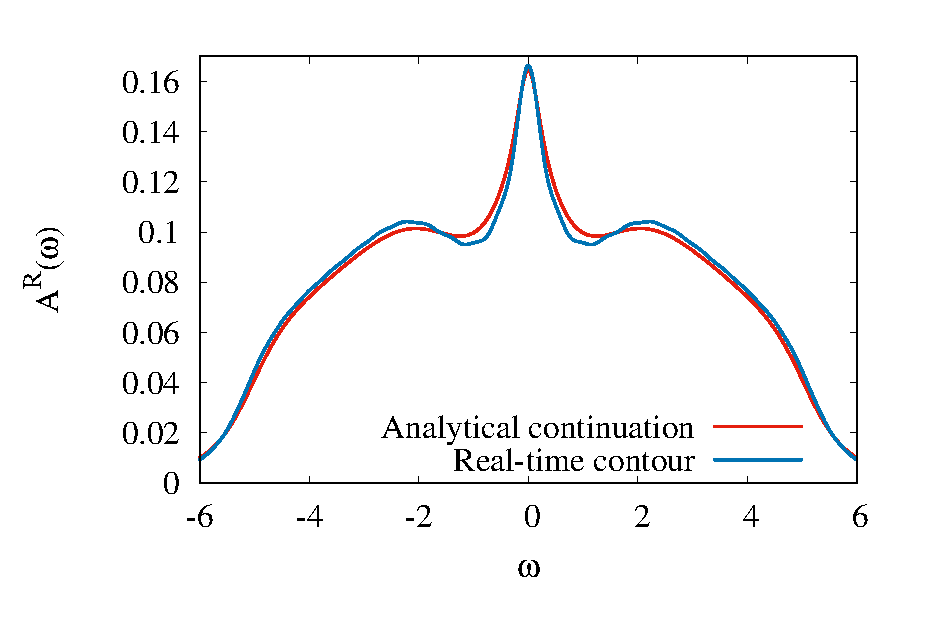
\includegraphics[width=0.5\linewidth]{Chapters/Theory_Kelgysh/figure/DOS_comp.eps}} 
\caption{Comparison of DMFT+TMA-PH spectral functions obtained using different methods ($U=2.88$)}
\label{Eq_comp_DOS}
\end{figure}

In \citep{PhysRevB.91.235114} systematic studies of the accuracy calculating the self-energy for the single-band model was found that in weak-coupling regime second order perturbation theory is more reliable than performing additional channals summations. It is also known that the magnetic part of the particle-hole channal has a divergence in the denominator, which does not allow us to use it in the standard form of the DMFT scheme for $U>0.3W$($W$-bandwidth). Based on these, further calculations for the single-band model in this work will be provide using 2D square lattice and IPT scheme. 
\begin{figure}[h!]
\begin{minipage}[h]{0.5\linewidth}
\center{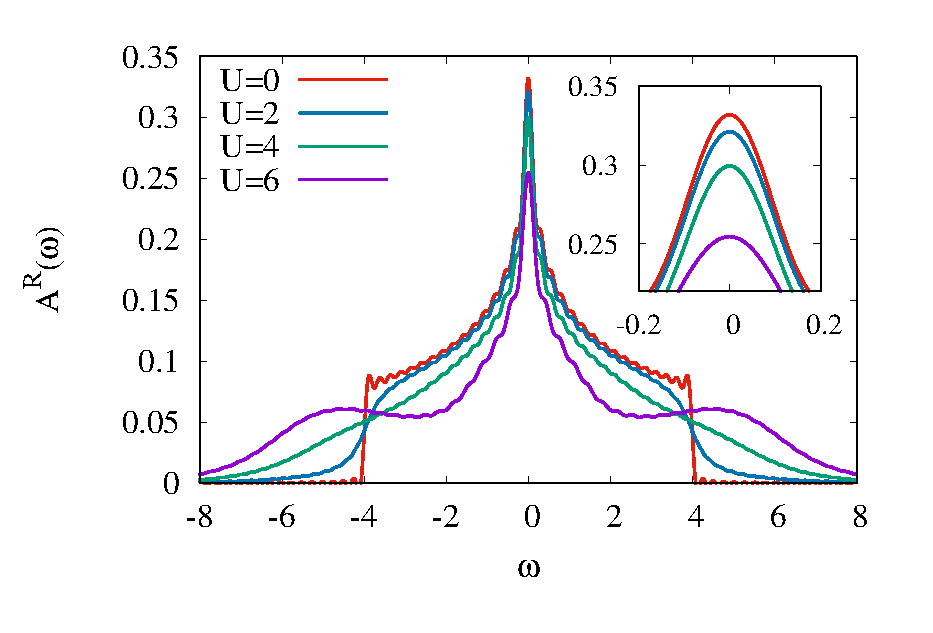
\includegraphics[width=1\linewidth]{Chapters/Theory_Kelgysh/figure/DOS_U.eps}} (a) \\
\end{minipage}
\hfill
\begin{minipage}[h]{0.5\linewidth}
\center{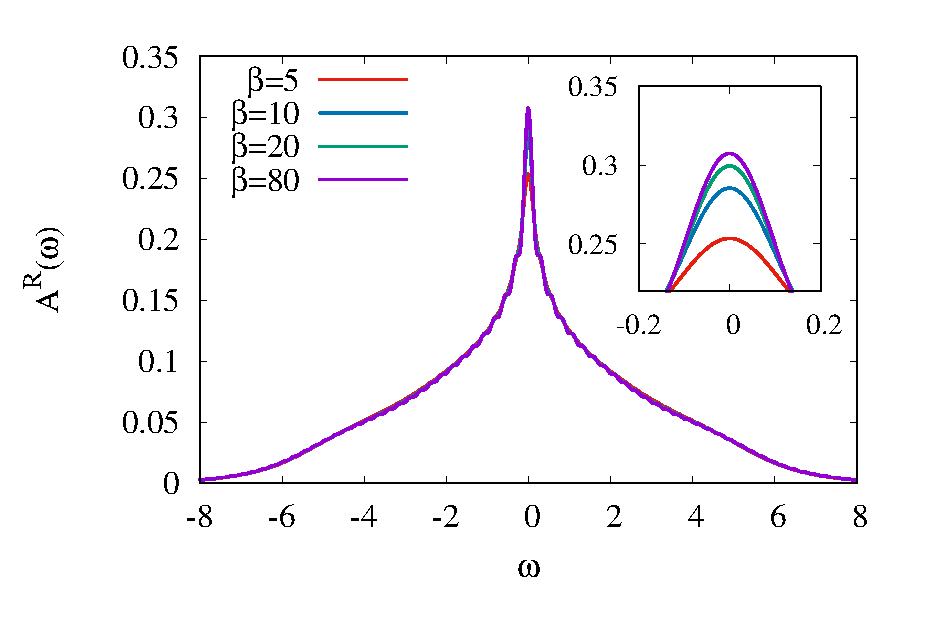
\includegraphics[width=1\linewidth]{Chapters/Theory_Kelgysh/figure/DOS_T.eps}} (b) \\
\end{minipage}
\caption{(a) IPT spectral function with different Coulomb interaction. (b) IPT spectral function with different inverse temperatures for $U=4$.}
\label{Eq_IPT_DOS}
\end{figure}

In Fig.~\ref{Eq_IPT_DOS}a equilibrium IPT spectral functions is characterized by different Coulomb interactions. Results for $U=0$ represent tight-binding model with $W=8$. With increasing interaction, we observe the disappearance of sharp edges and the gradual blurring of the density of states, which leads to an increase in the bandwidth. In a high $U=6$, the formation of three peak structures could be observed, which is present in the $U \sim W$ region. Decreasing temperature not significantly increase the peak height at $\omega=0$ (Fig.~\ref{Eq_IPT_DOS}b).

\FloatBarrier


\section{\label{PP_s}Appendix: Pump-probe spectroscopy}

Ultrafast time scale processes characteristic for a large number of physical phenomena, thereby induce great interest in fundamental and applied physics. The pump-probe spectroscopy \citep{Petek_Ogawa_1997,Axt_2004_Kuhn,ABRAMCZYK2005147} is the powerful and widely used experimental technique to study such nonequilibrium phenomena. Observation of fast processes is crucial to understanding ultrafast phase transitions, dynamics of various excitations, and many scattering processes.

%\citep{Zewail_Ahmed_2000,Petek_Ogawa_1997,Axt_2004_Kuhn}


%2) Схема эксперимента

\begin{figure}[h!]
\center{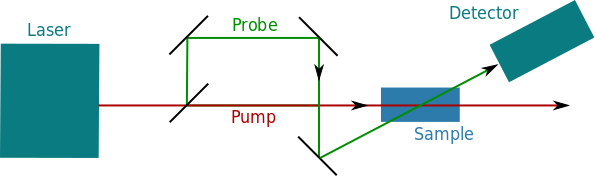
\includegraphics[width=0.6\linewidth]{Chapters/introduction_1/figure/PP_scheme.png}} \\
\caption{Schematic setup of the pump-probe spectroscopy.}
\label{fig:PES_scheme}
\end{figure}

In Fig.~\ref{fig:PES_scheme}, is shown a schematic picture of the pump-probe spectroscopy measurements. To study dynamical processes, the system must be perturbed from an equilibrium state to an excited one by using the "pump" beam. The excitement of the sample is possible with various parameters of the pump pulse including duration, intensity, polarization, and energy. Another higher frequency "probe" pulse is used to observe a transient response after the pump. Both pulses approach the sample on different paths determined by the arrangement of mirrors, which allow obtaining time-resolved data for physical quantities.

%3) Физика процесса
The distribution of photoelectrons in energy, angle and time gives information about the evolution of the electronic structure due to perturbation of the system. 
Access to nonequilibrium states of matter attainable through femtosecond IR \citep{C9CP00855A, PhysRevApplied.3.051002}, optical \citep{Steinmeyer1507, Hentschel_2001} or extreme ultraviolet lasers (EUV) and X-ray free
electron lasers \citep{McNeil_2010,Dunne_Mike_2018,Parra2003,Maltezopoulos_2008}.
At the moment, a large number of experiments and studies has been done for various materials: correlated insulators \citep{PhysRevLett.112.087402,PhysRevB.89.205114,PhysRevLett.113.216401}; graphene \citep{Nature_Materials_12_1119_1124,doi:10.1063/1.4871381} and graphitic materials \citep{PhysRevLett.76.483,PhysRevLett.87.267402,PhysRevLett.112.257401,PhysRevB.92.184303}; semiconductors \citep{RevModPhys.83.543,PhysRevB.81.113203}; cuprate superconductors \citep{PhysRevLett.99.197001,PhysRevLett.107.097002,Smallwood1137,Sci_Rep_6_18747_2016}; topological insulators \citep{Wang453,Sci_Rep_5_13213_2015,PhysRevLett.108.117403,PhysRevLett.109.127401,Nat_Commun_5_3003_2014,Sci_Rep_5_8160_2015,PhysRevLett.115.116801}; ultracold atoms \citep{PhysRevA.50.5025,PhysRevA.64.033421,PhysRevA.80.033404,}.




\clearpage
\bibliographystyle{abbrvnat}
\bibliography{references}
\end{document}
